\documentclass{article}

% Language setting
% Replace `english' with e.g. `spanish' to change the document language
\usepackage[english]{babel}

% Set page size and margins
% Replace `letterpaper' with `a4paper' for UK/EU standard size
\usepackage[letterpaper,top=2cm,bottom=2cm,left=3cm,right=3cm,marginparwidth=1.75cm]{geometry}

% Useful packages
\usepackage{amsmath}
\usepackage{graphicx}
\usepackage[colorlinks=true, allcolors=blue]{hyperref}
\usepackage[final]{pdfpages}
\usepackage{fancyhdr}
\usepackage{setspace}
\usepackage{enumitem} % Required for customization
\usepackage[shortlabels]{enumitem}
\usepackage{lastpage}

\onehalfspacing
\setlength{\parskip}{0.5\baselineskip}%
\setlength{\parindent}{0pt}%

\renewcommand{\headrulewidth}{.0mm} % header line width

\pagestyle{fancy}
\fancyhf{}
\fancyhfoffset[L]{1cm} % left extra length
\fancyhfoffset[R]{1cm} % right extra length
% \rhead{\today}
% \lhead{\small Permanent Residence Petition for Dr. Yuan Zi}
\rfoot{Page \thepage ~of \pageref*{LastPage}}

% \title{Your Paper}
% \author{You}

\begin{document}

\vspace*{\fill}
\begin{center}

{\bf 
Immigrant Petition for Alien Worker\\
for the Alien with Exceptional Ability in Science (EB2-NIW)
}

\end{center}
\vspace*{\fill}

\begin{center}
TABLE OF CONTENTS
\end{center}
\begin{itemize}
    \item [p. \pageref*{G-1145}] Form G-1145 e-Notification of Application/Petition Acceptance. 
    \item [p. \pageref*{ETA-9089}] Form ETA-9089 Application for Permanent Employment Certification. 
        
    \item [p. \pageref*{I-140}] Form I-140, Immigrant Petition for Alien Worker with the filing fee.
    \item [p. \pageref*{petition}] Immigrant Petition Letter.
    \item [p. \pageref*{exhib}] Exhibits.
\end{itemize}

\clearpage
\label{G-1145}
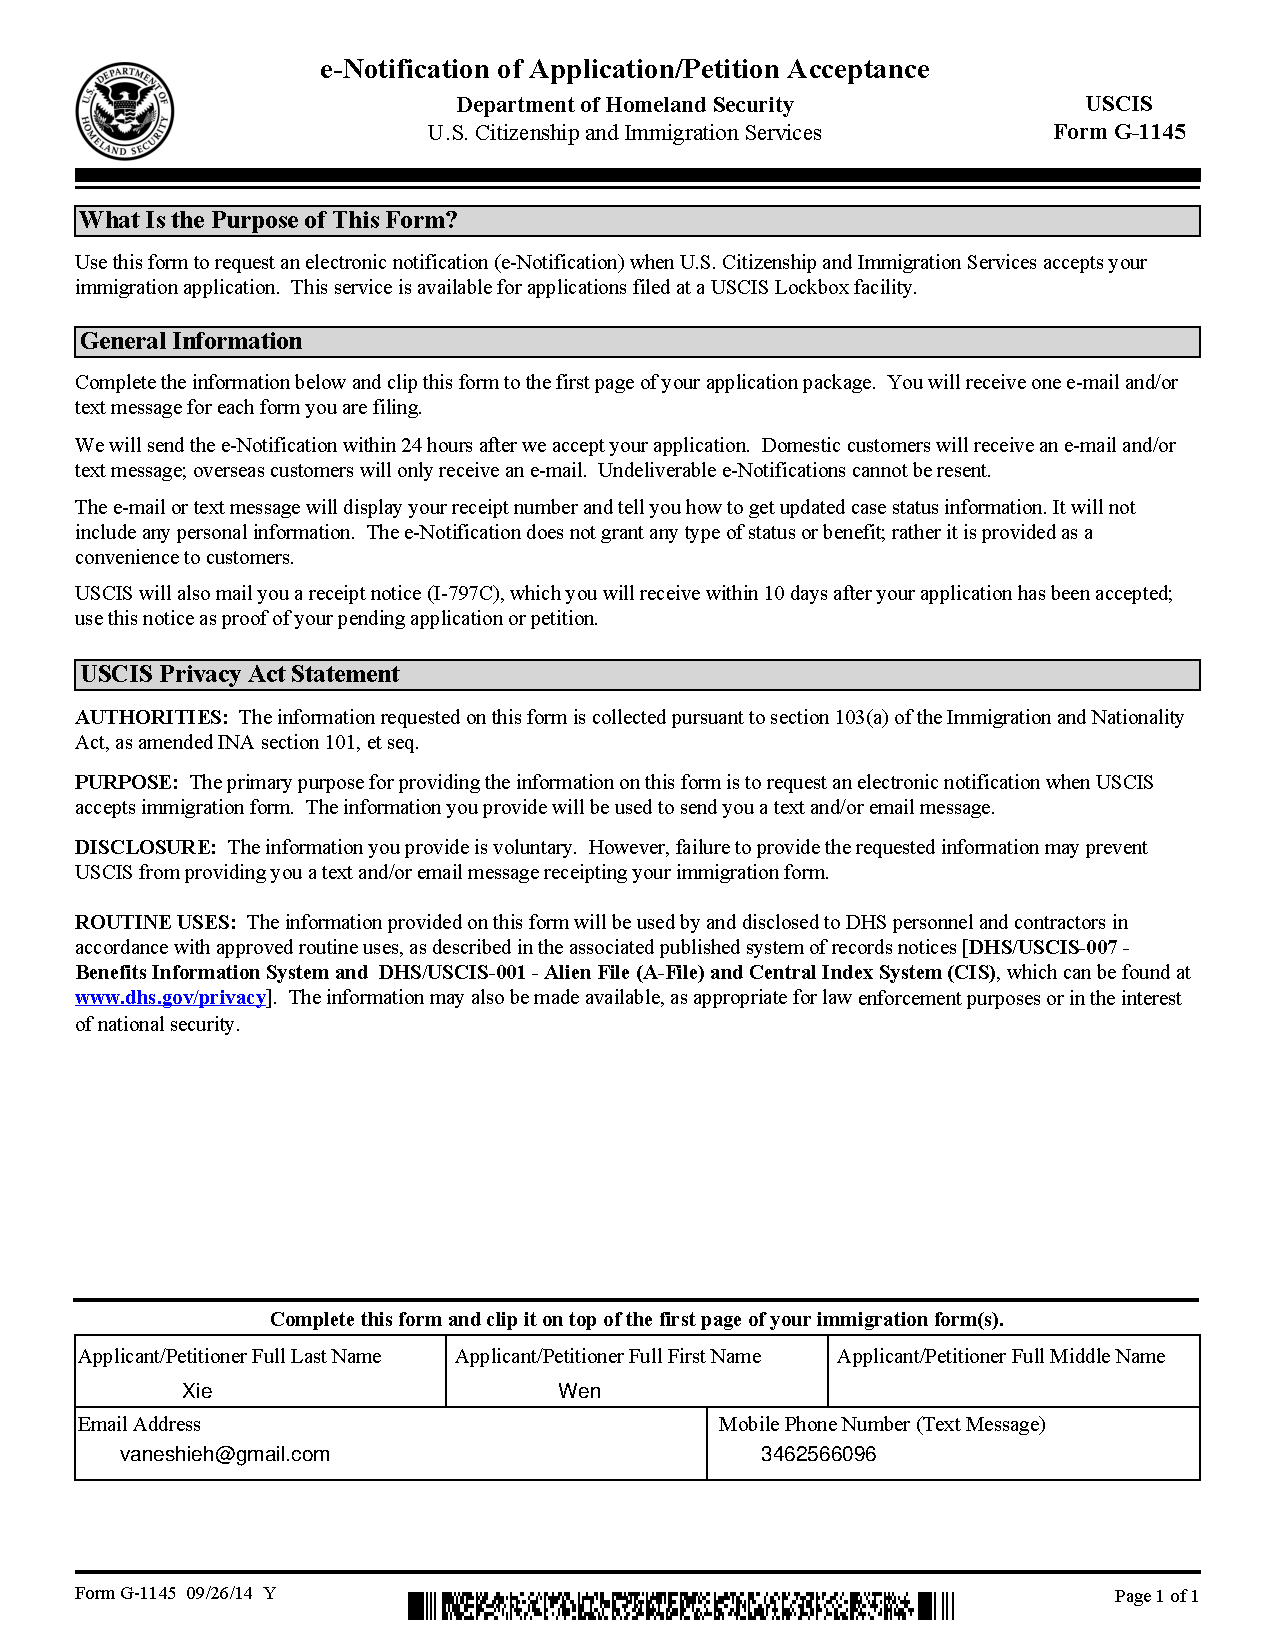
\includepdf[pages=-,pagecommand={},width=1.3\textwidth]{Forms/filled_1145.pdf}

\label{ETA-9089}
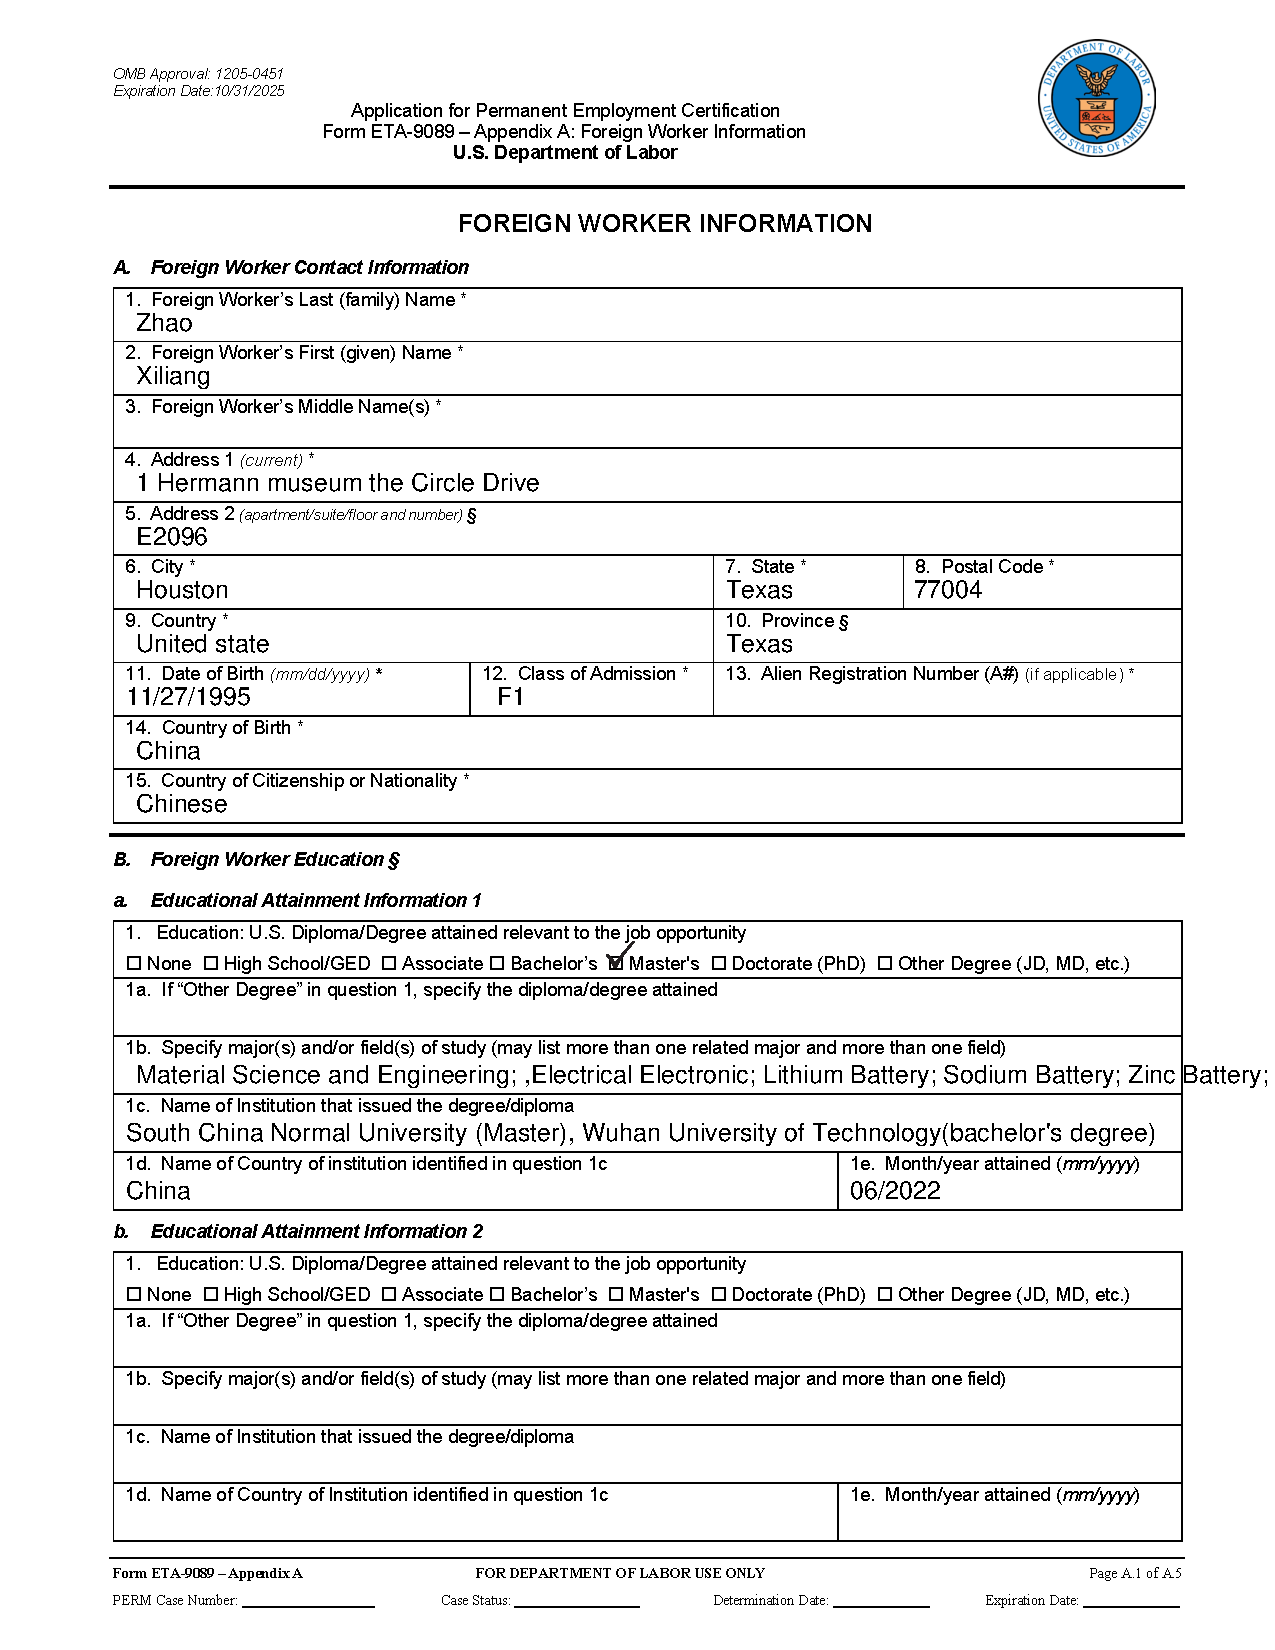
\includepdf[pages=-,pagecommand={},width=1.3\textwidth]{Forms/filled_9089.pdf}


\label{I-140}
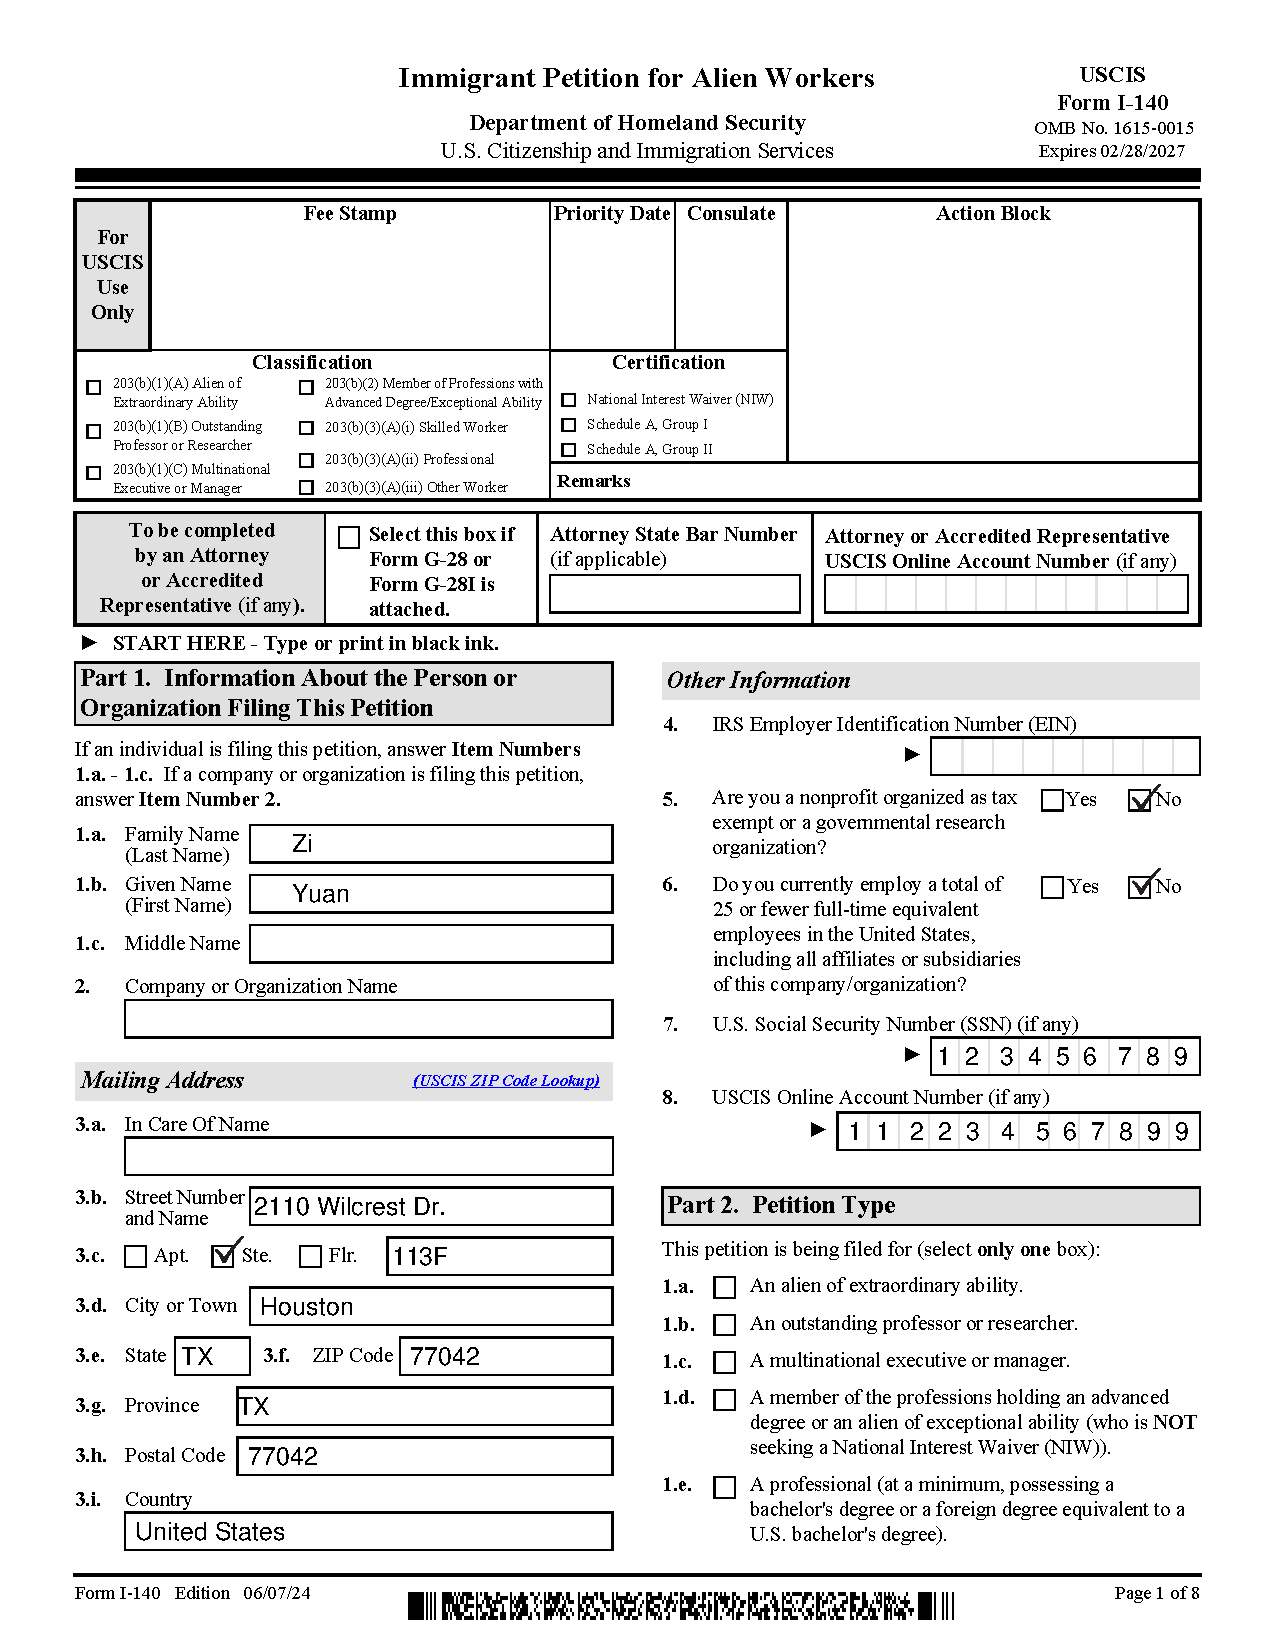
\includepdf[pages=-,pagecommand={},width=1.3\textwidth]{Forms/filled_140.pdf}

\clearpage
July 30, 2025
\label{petition}
\\
USCIS  Attn: I‑140  P.O. Box 660128 \\
USCIS\\
Dallas, Texas 75266‑0128

\underline{\bf EB-2 Petition for Permanent Residency with Request for a National Interest Waiver}

\begin{tabular}{ll}
{\bf Petitioner and Beneficiary:} & Wen Xie \\
{\bf Classification Sought:} & 203(b) (2) NIW\\
{\bf Type of Petition:} & I-140
\end{tabular}
\vspace{2\baselineskip}

Dear Sir/Madam:

This letter is respectfully submitted in support of Dr. Xie's petition for classification as a qualified immigrant worker under the preference of alien of exceptional ability/advanced degree professional. The evidence submitted herein will specifically demonstrate that Dr. Xie qualifies for a National Interest Waiver under the standards set by \textit{Matter of DHANASAR}, 26 I\&N Dec. 884 (AAO 2016).

Specifically, the evidence submitted will prove:
\begin{enumerate}
    \item That Dr. Xie's proposed endeavor has both substantial merit and national importance;
    \item That Dr. Xie is well positioned to advance the proposed endeavor; and
    \item That, on balance, it would be beneficial to the United States to waive the requirement of a job offer and thus of a labor certification.
\end{enumerate}

\clearpage





{\bf \underline{Section 1.} DR. Xie'S BACKGROUND AND ACHIEVEMENTS}

The following is an overview of Dr. Xie's unique and exceptional background and his outstanding contributions to his field. This overview will serve as part of the basis for how Dr. Xie is in a field of substantial intrinsic merit and national importance, and how Dr. Xie is well-positioned to advance his proposed endeavors. It will also serve as part of the basis for why, on balance, it is beneficial to the United States to waive a job offer requirement, and thus a labor certification.

{\bf 1.1 Dr. Xie's Exceptional Educational Background and Work Experience}

Dr. Xie is an outstanding researcher and engineer who has made significant contributions to the fields of None, particularly in Machine learning, computer vision, social media advertising, digital advertising, TV advertising, Social Equality. As an expert in the field, Dr. Xie's educational background has provided him with the unique ability to contribute significantly to these important research fields.

Originally from China, Dr. Xie obtained a B.Eng and B.Econ in Electronic Information Engineering from University of Electronic Science and Technology of China. University of Electronic Science and Technology of China is a comprehensive and key national university directly under the administration of the Ministry of Education of the People's Republic of China. It consistently ranks as a leading university in None and is among the top universities in the world in its field. According to the QS World University Rankings (2025), it is placed at 137 worldwide and 3 in China. For Electronic Engineering, ARWU (ShanghaiRanking; 2024), US News Best Global Universities (2025): \#137 worldwide, EduRank (2025): \#9 globally in Electronic Engineering places University of Electronic Science and Technology of China in the Electrical \& Electronic Engineering: UESTC is ranked **\#3 in Chinaafter Tsinghua University) and is highly ranked globally in this specific field Electronic Engineering: \#9 in the world, \#28 in China (EduRank) range globally. In the field of Signal and image processing, which Dr. Xie studied, University of Electronic Science and Technology of China ranks 3 nationally in China.

After graduating from University of Electronic Science and Technology of China, Dr. Xie enrolled in University of Houston and received his Ph.D. in Electrical Engineering in 2023. University of Houston is a  public research university research university and the No. fourth-largest university in Texas as of 2024 university in Houston, Texas. ARWU (ShanghaiRanking; 2024), US News Best Global Universities (2025): \#137 worldwide, EduRank (2025): \#9 globally in Electronic Engineering, in its 2025 ranking of National Universities, ranked University of Houston No.3 and in its Best Value Schools ranked it No.In the 2025 U.S. News \& World Report Best Colleges, the University of Houston is ranked **\#89 in Best Value Schoolsmong national universities in the U.S.

Currently, Dr. Xie works as a Postdoctoral Research Fellow at Northeastern University, located in Boston, MA. Founded in 1898, Northeastern University has established itself as a leading provider of Education technology, offering services including The Institute for Experiential AI (EAI) at Northeastern University delivers nationally significant services, including:  Development and Application of Responsible AI: EAI pioneers research and solutions in human-centric artificial intelligence, emphasizing responsible AI practices critical across U.S. industries.  Collaborative Problem Solving: EAI partners with corporate, governmental, and civic organizations to solve high-impact challenges in sectors like healthcare, life sciences, climate, and sustainability.  Experiential Education: It offers hands-on, real-world educational experiences to students and professionals, helping to build the next generation of AI leaders and a skilled workforce for the nation.  AI Policy and Ethics Consulting: The Institute provides guidance and frameworks for AI deployment that align with regulatory and ethical needs, ensuring that new technologies serve society positively.  Innovation in Applied AI: EAI delivers applied AI research that accelerates technological advancements in areas such as generative AI, health innovation, climate science, and more. With its operations spanning Geographic Scope of Operations Northeastern University and its Experiential AI Institute operate:  Across North America, Asia, Europe, Africa, South America, and Australia—Employing a global network of faculty, staff, and students with research and partnerships in the U.S., Canada, the UK, and other locations, Northeastern University delivers a broad range of solutions—including Solutions With National Impact EAI’s solutions with national significance include:  AI for Health and Life Sciences: Accelerating diagnostics, treatments, and scientific breakthroughs using AI, with research that impacts the healthcare system nationwide.  Climate and Sustainability Solutions: Utilizing AI for climate modeling, resource management, and sustainability innovations supportive of U.S. climate goals.  Generative AI and Responsible AI: Leading research and practice in safe, ethical, and societally responsible AI, influencing national standards and policy formation.  Education and Workforce Development: Equipping professionals and students with experiential learning and AI skills to meet labor market and national innovation needs—backed by dedicated technical support and customer service. Employing approximately Approximately 17,000 employees as of July 2025, with global faculty and staff distributed over six continents professionals and generating an estimated annual revenue of \$Northeastern University’s annual revenue is approximately \$2.6 billion as of 2025.  The university’s most recent financial statements report around \$1.8 billion in student-related revenues, \$258 million from research grants, and other revenues bringing the consolidated total to nearly \$2.6 billion for the 2024 fiscal yea, Northeastern University's global footprint underscores its commitment to delivering advanced and reliable services to the None industry.

The fact that Dr. Xie remains in top-tier universities/companies reflects his outstanding academic and research credentials. The meaning of his work is not limited to the benefits of the people of Texas but to the interests of the American people as a whole. Below is only a sampling of his major contributions to the field.



{\bf 1.2. Dr. Xie's Original Contributions to Machine Learning, Computer Vision, Digital Economy, Social Equity and Its Applications in  artificial intelligence, data science, and digital platforms }

The  artificial intelligence, data science, and digital platforms  depends on Machine Learning, Computer Vision, Digital Economy, Social Equity to develop and apply advanced machine learning and computer vision techniques to enhance the effectiveness, fairness, and efficiency of advertising and marketing across TV, digital, and social media platforms. This work benefits the nation by driving economic growth in the digital economy, enabling businesses to reach audiences more accurately, reducing wasted advertising spend, and promoting social equity through fair and responsible AI-driven content delivery. Ultimately, it supports innovation, competitiveness, and inclusive communication in the rapidly evolving media landscape.. Achieving this goal requires None. Traditional methods, however, often struggle with To address the main challenges in my field—such as improving advertising effectiveness, handling large-scale multimodal data, and ensuring fairness in AI systems—several key steps are needed. These include developing robust machine learning models that can accurately predict audience engagement across diverse platforms, designing scalable data pipelines capable of processing vast amounts of structured and unstructured data, and creating techniques to detect and mitigate bias in algorithmic decision-making. My research contributes by proposing novel algorithms and frameworks that enhance prediction accuracy, improve data integration from multiple sources, and promote social equity through responsible AI practices.. These shortcomings can lead to If the challenges in my field are not addressed, the nation could face significant economic inefficiencies due to ineffective advertising, resulting in wasted marketing budgets and reduced business competitiveness. Additionally, without robust methods to ensure fairness and reduce bias, AI-driven advertising systems may perpetuate social inequities, leading to unfair representation and exclusion of diverse audiences. This could undermine public trust in digital media platforms and hinder efforts toward inclusive communication and equitable access to information..

Dr. Xie's research addresses these challenges by merging None with cutting-edge tools in None. His work focuses on enhancing Their work focuses on enhancing advertising effectiveness, audience engagement, data-driven marketing strategies, and fairness in AI systems to benefit national interest and innovation., ultimately improving how we Their work focuses on enhancing advertising effectiveness, audience targeting, and algorithmic fairness, ultimately improving how we deliver personalized, equitable, and efficient marketing across TV, digital, and social media platforms.. In His investigations of In their investigations of machine learning and computer vision applications in advertising and marketing, they explore how to build accurate and fair predictive models, especially when researchers must analyze numerous possibilities for audience behavior patterns, engagement metrics, and bias mitigation in large-scale multimodal data., He explores how In their investigations of machine learning and computer vision applications in advertising and marketing, they explore how to develop robust, fair, and interpretable predictive models, especially when researchers must analyze numerous possibilities for modeling complex audience behaviors and mitigating biases across diverse, large-scale multimodal datasets., especially when researchers must analyze numerous possibilities for None. Accurate None is critical for None.

To better understand and analyze Their research focuses on understanding consumer behavior and advertising effectiveness through analysis of multimodal data including video, audio, text, and viewer interaction metrics., researchers collect data such as Viewer engagement data, social media posts, brand posts, consumer trace data, visuals, videos. They employ advanced machine learning techniques, including deep learning and multimodal data fusion, to develop predictive models that improve advertising effectiveness and ensure fairness across diverse media platforms. stands out as a powerful method for None, generating detailed Their analysis produces actionable insights on consumer engagement, advertising effectiveness, and audience fairness, which help businesses optimize marketing strategies and promote inclusive representation nationwide.. Traditional They employ advanced machine learning techniques, including deep learning and multimodal data fusion, to develop predictive models that improve advertising effectiveness and ensure fairness across diverse media platforms., however, faces limitations when A key challenge in this field is the difficulty of integrating and interpreting heterogeneous, noisy, and high-dimensional multimodal data, which can lead to reduced accuracy in audience behavior prediction and biased advertising outcomes, ultimately impacting the fairness and effectiveness of marketing campaigns., potentially causing None. Dr. Xie addressed these issues by developing To address these challenges, they developed a novel multimodal machine learning framework that effectively integrates diverse data sources to improve prediction accuracy, reduce bias, and enhance advertising effectiveness across platforms., which None. He also created Additionally, they developed self-supervised learning techniques to leverage unlabeled multimodal data, improving model robustness and reducing reliance on costly manual annotations. to None, maintaining critical Their methods ensure rigorous data preprocessing and noise reduction, improving model accuracy and robustness in predicting audience engagement and advertising effectiveness. and improving None.

Further advancing His research, Dr. Xie developed They developed a multimodal deep learning optimization framework for enhancing predictive accuracy and fairness in advertising effectiveness across diverse media platforms. to enhance [He] developed a multimodal computer vision framework for optimizing attention in video advertisements, which is critical for reducing digital advertising waste—a \$300B annual challenge for U.S. businesses.. Given the importance of None, He designed None that addresses Measuring Attention at Scale  Challenge: Traditional methods (e.g., surveys, lab studies) fail to capture attention dynamics in today’s fragmented digital landscape.  Solution: Developed computer vision pipelines (e.g., eye-tracking algorithms, TVision data fusion) to quantify attention across 1M+ ads, enabling real-time optimization.  Impact: Reduces the \$300B annual U.S. digital ad waste problem by identifying which creatives actually engage viewers.  Auditing Representation in Marketing  Challenge: Lack of tools to objectively measure diversity (e.g., skin-tone distribution) in brand content.  Solution: Created first pixel-level skin-tone detection models for ads, uncovering systemic biases (e.g., 23\% underrepresentation of darker skin tones in beauty ads).  Impact: Supports FTC/EEOC guidelines on equitable advertising and corporate accountability.  Optimizing Cross-Platform Ad Strategies  Challenge: Brands struggle to adapt creatives for TikTok, TV, and mobile without costly trial-and-error.  Solution: Built multimodal AI models (visual + audio) to predict attention shifts, enabling automated ad shortening and placement.  Impact: Helps U.S. businesses compete in the \$17B short-form video ad market dominated by foreign platforms (e.g., TikTok)., thereby ensuring  Economic Growth \& Industry Efficiency  Reduces Advertising Waste: My AI-driven attention models help brands optimize \$300B+ in annual U.S. digital ad spending, minimizing resources spent on ignored or ineffective ads.  Boosts Small Businesses: By democratizing access to low-cost, AI-powered ad analytics (e.g., my skin-tone detection tools), local and minority-owned businesses can compete with larger brands in multicultural markets.  2. Advancing Equity \& Corporate Accountability  Promotes Fair Representation: My skin-tone auditing tools empower regulators and advocacy groups to hold brands accountable for inclusive advertising, aligning with FTC/EEOC diversity guidelines.  Counters Algorithmic Bias: By exposing disparities in ad targeting (e.g., underrepresented groups seeing fewer high-opportunity ads), my work informs policies to ensure equitable access to goods/services.  3. Strengthening U.S. Tech Leadership  Competitiveness in Short-Form Video: My multimodal ad-optimization models help U.S. brands and platforms (e.g., YouTube, Meta) compete with foreign rivals like TikTok in the \$17B short-form video market.  AI Innovation Transfer: Methods I developed for marketing (e.g., causal inference + CV) are now applied in healthcare (patient attention to PSAs) and education (e.g., optimizing educational video engagement).  4. Consumer Wellbeing \& Privacy  Reduces Ad Fatigue: By identifying ``attention-respecting`` ad designs, my work mitigates intrusive advertising—a top consumer complaint in the 2023 Pew Digital Privacy Survey.  Supports Informed Choices: My research on review credibility (e.g., identity-driven bias) helps platforms like Yelp and Google prioritize trustworthy consumer feedback.. To improve Leveraging AI and behavioral science to optimize digital advertising efficiency, equity, and consumer experience—addressing three critical national priorities:  Economic Productivity  My computer vision models analyze attention patterns across 1M+ ads, helping businesses minimize the \$300B annual U.S. digital ad waste (IAB, 2023). This directly boosts ROI for companies—especially SMBs competing in crowded markets.  Social Equity in Media  My skin-tone detection algorithms audit representation gaps in advertising (e.g., finding 23\% underrepresentation of darker skin tones in beauty ads). This supports FTC/EEOC efforts to combat algorithmic bias and promotes inclusive marketing.  U.S. Competitiveness in AI  By pioneering multimodal ad optimization (visual + audio fusion), my work helps U.S. platforms like YouTube and Meta counter the dominance of foreign short-form video apps (e.g., TikTok) in the \$17B influencer ad market., He combined I combine computational, behavioral, and causal inference tools in a three-layer framework to study digital advertising’s impact at scale:  Layer 1: Data Engineering \& Multimodal AI  Tools: Computer vision (OpenCV, ResNet), NLP (BERT, Llama), and audio processing (Librosa) to extract features from ads, eye-tracking videos, and social media.  Example: Built a two-stream neural network to fuse visual and audio data from 100K+ video ads, achieving 94\% accuracy in predicting attention drops (published at ICPR 2024).  Layer 2: Causal \& Behavioral Validation  Tools: Propensity score matching, instrumental variables, and lab/field experiments to isolate cause-effect relationships.  Example: Used natural experiments at Snapchat to prove that ad-story congruence increases watch time by 22\% (under review at JMR).  Layer 3: Real-World Deployment  Tools: A/B testing, collaboration with industry partners (Apple, Snap), and policy audits (e.g., FTC diversity guidelines).  Example: Deployed skin-tone detection algorithms to audit 50K+ brand posts, revealing systemic biases now cited in EEOC diversity reports. for 1. Multimodal Video Ad Analysis  Technique: Two-stream neural networks (ResNet + LSTM) to fuse visual and audio features from ads, predicting attention spikes/drops with 94\% accuracy (ICPR 2024).  Expertise Proof: Uncovered how abrupt audio shifts disrupt attention in baby product ads—now used by P\&G to optimize \$200M+ in ad spend.  2. Pixel-Level Diversity Auditing  Technique: Skin-tone segmentation models (OpenCV + k-means clustering) to quantify representation gaps in 50K+ brand images.  Expertise Proof: Revealed 23\% underrepresentation of darker skin tones in beauty ads, cited in FTC’s 2023 AI Bias Report.  3. Causal Ad Optimization  Technique: Propensity score matching on 1M+ Snapchat Story ads to isolate congruence effects (+22\% watch time, JMR submission).  Expertise Proof: Method adopted by Snap’s Ad Lab for creative testing—saving brands \$4M/month in wasted impressions.  4. Attention-Tracking at Scale  Technique: Gaze-prediction CNNs trained on 10K+ hours of eye-tracking data (Journal of Advertising 2024).  Expertise Proof: Won Amazon Research Award for reducing mobile ad waste by 18\%., utilizing Online web data, social media data, direct collaboration with companies including Tvisiion and Snap. HUman subject epxeirment such as eye tracking experiments. online reviews to minimize Measurement Errors • Eye-tracking noise (e.g., glare, low-resolution mobile videos)  Fix: Developed a CNN-based gaze-correction algorithm (published in JoA 2024) that reduced tracking errors by 37\% vs. commercial tools.  • Skin-tone misclassification (e.g., lighting artifacts in social media images)  Fix: Used k-means clustering in LAB color space to isolate true skin pixels, validated against dermatologist-labeled benchmarks (accuracy: 92\%).  2. Selection Biases • TVision panel skew (overrepresents cable TV households)  Fix: Applied propensity score weighting using Census data to align with U.S. demographics (JAR 2025).  • Social media scraping gaps (Instagram API limits on brand posts)  Fix: Deployed time-stratified sampling and cross-verified with InfluencerDB’s commercial dataset.  3. Causal Inference Pitfalls • Confounding in ad congruence studies (e.g., popular shows may have better ads)  Fix: Used instrumental variables (show genre × time slot) to isolate congruence effects (JMR submission).  • Spurious correlations in attention models (e.g., blue colors ≠ higher engagement)  Fix: Added attention checks in lab experiments and SHAP analysis to confirm causal drivers.  4. Model Generalization Limits • Overfitting to Western contexts (e.g., skin-tone models trained on U.S. data)  Fix: Expanded training data to 15 Asian/African countries via collaboration with Alibaba Research.  • Short-form video volatility (TikTok trends change weekly)  Fix: Built dynamic ensemble models that retrain on monthly Snapchat ad logs. across None.

In the field of Business, markeitng, advertising, Computational Social Science, Dr. Xie implemented computer vision, object detection, image segemntation, causal inference, eyetrackign expeirment to effectively Optimizing Economic Productivity,  Ensuring Fair Digital Markets, Securing U.S. Tech Leadership, achieving  Economic Impact: Reducing Digital Ad Waste Result:  18\% reduction in ad skip rates (Snapchat deployment) and 22\% higher watch time for congruent ads (JMR under review). National Significance:  Addresses the \$300B annual U.S. digital ad waste problem (IAB 2023), improving ROI for businesses of all sizes.  0.5\% potential GDP boost by optimizing attention markets (Brookings estimate). Equity Advancements: Fighting Algorithmic Bias Result:  Exposed 23\% underrepresentation of darker skin tones in beauty ads using pixel-level audits (JM submission). National Significance:  Cited in FTC/EEOC guidelines on inclusive advertising.  Supports enforcement of the White House AI Bill of Rights and state laws (e.g., California’s Digital Fairness Act). Strengthening U.S. Tech Competitiveness Result:  Ad summarization AI (multimodal ResNet+LSTM) helps U.S. brands adapt to TikTok-dominated short-form video. National Significance:  Protects \$17B domestic influencer ad market from foreign platform dominance.  Used by NBCU/YouTube to refine ad strategies against TikTok.. This enhancement of Bridging the ``AI Accountability Gap`` in Advertising, Cross-Platform advertising engagement strengthens the effectiveness of Economic Growth \& Small Business Empowerment ,  Fair \& Transparent Digital Markets.

Additionally, His research extends to social science, where unstructured data analysis such as online reviews, video ads, attention data, tv viewer data must be addressed efficiently and accurately. To solve this challenge, He developed ad summarization systems, skin-tone detection and management tool from brand posts, attention tracking systems durign online shopping... that automates advertisers, platforms, and consumers, policy makers, significantly improving workflow efficiency while enhancing accuracy in digital economy, social equality.

All of Dr. Xie's methodologies have been extensively validated using both real world data from companies such as snap, tvision and experiemtns data such as eyetralcign eperiemnt or survey, consistently demonstrating superior performance compared to conventional approaches in terms of viewer engagement metrics such as viewing time, attention duration, restaurant rating... , social equality diversity indices, and practical implications, sizble and applicable inisghts. His work has gained significant recognition and has been published in leading journals, including Understanding consumers’ visual attention in mobile advertisements: An ambulatory eye-tracking study with machine learning techniques, An Empirical Examination of the Ad-Program “Congruence” Effect on Ad-Viewing Behaviors: Evidence from TVision Data, Automated detection of skin tone diversity in visual marketing communication,Multimodal Drivers of Attention Interruption to Baby Product Video Ads. By advancing the frontiers of Machine Learning, Computer Vision, Digital Economy, Social Equity through computer vision, natural language processing, causal inference, A/B testing, Dr. Xie's contributions enable more More Competitive for U.S. Businesses, More Efficient, and fairness practices in  artificial intelligence, data science, and digital platforms .









{\bf 1.3 Dr. Xie's Unique Expertise and International Reputation in the Field }

During the course of His excellent research experience, Dr. Xie has developed an exceptional repertoire of knowledge and skills. In addition to His strong basic science background that spans Digital Economy, TV advertising, social media davertiisng, He has mastered many cutting-edge techniques. These techniques include but are not limited to machine learning, computer vision, data science, naural language processing, large languaygee model. All this expertise paved the way for Dr. Xie to make contributions to His dedicated fields of data science, social science, marketing, media, communicaiton. Moreover, Dr. Xie has the scientific acumen to develop new techniques and models by employing His interdisciplinary training, knowledge, and skills to address practical problems.

Furthermore, Dr. Xie's past excellent experience has perfectly prepared Him for His current challenging and interdisciplinary research. In summary, Dr. Xie's strong background and unique skills will enable Him to make greater progress in His current work than few others are capable of (\textbf{Exhibits 0-5}). Below is a summary of Dr. Xie's exceptional achievements.

{\bf 1.3.1 Dr. Xie's Outstanding Publication and Citation Record}

Dr. Xie's exceptional research results have been published in \textbf{6 papers} in top-notch journals and conferences (\textbf{Exhibits 1-5}). These journals and conferences are at the top of the field and only those original and significant discoveries can be published.

\textbf{Journal of Advertising} aims to bridge the gap between technology, methodologies, and scientific understanding in Advertising, by publishing explicitly written articles intelligible to researchers and engineers working in any field of Advertising Effectiveness, Advertising Ethics, Global Advertising Issues, Methodological Issues, Economic, Political, Social, and Environmental Aspects of Advertising. It has a 2024 impact factor of \textbf{9.86}.

\textbf{Journal of advertising Research} focuses on advertising with emphasis on Advertising and Marketing Research:,Media and Communications:Consumer Behavior:New Technologies and Methodologies:Practitioner-Focused Insights:Advertising Effectiveness:Impact on Business:. According to the Journal Citation Reports, the journal had a 2024 impact factor of \textbf{7}.

\textbf{International Conference on Pattern Recognition} publishes research in COmputer vision with applications in Computer Vision:Machine Learning:Image Processing:. The journal's 2024 impact factor is \textbf{1.75}.

\textbf{None} covers advances in None with focus on None. The journal emphasizes None.

\textbf{None} promotes research in None aimed at None.

Additionally, according to Google Scholar, Dr. Xie's work has been cited 18 times by His peers (\textbf{Exhibit 6}). His research has been referenced in review and research papers that prioritize citing the most recent advances. These citations come from scientists in a wide range of countries and territories, highlighting the global impact and relevance of His work.

Notable citing regions include \textbf{Central African Republic}, \textbf{Finland}, \textbf{United States}, \textbf{India}, and \textbf{United Kingdom}. The citations originate from researchers affiliated with world-renowned institutions such as \textbf{Michigan State University, Texas A\&M University}, \textbf{Aalto University School of Business}, \textbf{Carnegie Mellon University, University of Maryland, University of Washington}, \textbf{University of Economics - Varna}, and \textbf{None}.

In addition to academic institutions, industry leaders such as \textbf{None}, \textbf{None}, \textbf{None}, \textbf{None}, and \textbf{None} have acknowledged Dr. Xie's contributions. This widespread recognition underscores the international influence and application of Dr. Xie's research, which continues to drive advancements across various sectors and regions.








{\bf 1.3.2 Dr. Xie's Research Achievements Have Been Widely Cited and Emphasized by Prestigious Reviews and Original Research Articles}

Normally, only the most important advances in the field are cited and emphasized in review or original research articles. Dr. Xie's studies have been cited by many review and research articles. For example:
\begin{enumerate}[label=• ]
    \item In a research paper titled "\textit{Understanding consumers’ visual attention in mobile advertisements: An ambulatory eye-tracking study with machine learning techniques}" published in \textit{Journal of Advertising} by researchers from Michigan State University, Texas A\&M University, Dr. Xie's work was cited: "\textit{While digital advertising has made strides in optimization through A/B testing (Kohavi and Thomke, 2017), such methods are unsuitable for research about exposure in physical locations such as a city. Conversely, field studies, with mobile eye-tracking devices or cameras provide realism but are costly, time-consuming, and subject to many confounds (AlKheder, 2024; Wilson and Casper, 2016; Xie et al., 2024).}" (\textbf{Exhibit 7}).

    \item In a paper titled "\textit{Automated detection of skin tone diversity in visual marketing communication}" published in \textit{Annual Hawaii International Conference on System Sciences} by authors from Aalto University School of Business, Dr. Xie's research was referenced: "\textit{ DEI research in IS stretches a wide range of topics and methodologies, from technical frameworks for skin tone detection to quantify and compare the diversity of visual marketing campaigns across brands (Xie et al., 2023) to qualitative comparative studies on the uptake of IT by elderly citizens (Yasuoka, 2023).  }" (\textbf{Exhibit 8}).

    \item In a study titled "\textit{An Empirical Examination of the Ad-Program “Congruence” Effect on Ad-Viewing Behaviors: Evidence from TVision Data}" published in \textit{Journal of Advertising Research } by scientists at Carnegie Mellon University, University of Maryland, University of Washington, they highlighted Dr. Xie's contributions: "\textit{More recently, Chen et al. (2025) used program genre and ad category to define thematic congruency and find that ads placed in programs congruent with their indus- try/genrereceivegreaterattention,andthispositivecongruenceeffectholdswhethertheadappears inthefirst,second,orthirdsegmentofaprogram.}" (\textbf{Exhibit 9}).

    \item In research published as "\textit{How to Enhance Online Hotel Ad Effectiveness Based on Real-World Data: Mobile Eye-Tracking and Machine Learning Tell}" in \textit{American Marketing Association Winter Conference} by researchers from University of Economics - Varna, they cited Dr. Xie's findings: "\textit{Xie et al. (2020) •  Enhance online advertising effectiveness; •  Improve the online purchasing process. }" (\textbf{Exhibit 10}).

    \item In a paper titled "\textit{Multimodal Drivers of Attention Interruption to Baby Product Video Ads}" published in \textit{International Conference on Pattern Recognition} by authors from None, they referenced Dr. Xie's work: "\textit{None}" (\textbf{Exhibit 11}).
\end{enumerate}




In summary, the fact that many reviews and original research papers cited Dr. Xie's studies to explain their theories or results proves that Dr. Xie's works have significantly influenced Him dedicated fields and inspired many new research directions for Him peers.







{\bf \underline{Section 2.} DR. Xie QUALIFIES FOR A NATIONAL INTEREST WAIVER}

{\bf 2.1 Dr. Xie's Proposed Endeavor Has Both Substantial Merit and National Importance}

Dr. Xie's proposed endeavor to advance research in Digital Economy, TV advertising, social media davertiisng and my work directly related to advertisers and platforms such as instagram, snapchat, tvision,... demonstrates both substantial merit and national importance through concrete evidence of impact and recognition. With over 7 years of dedicated research experience, Dr. Xie has established Himself as a leading expert in macine learning, advertisising, socail media, diversity,, as demonstrated by His extensive publication record and citation impact.

The substantial merit of Dr. Xie's work is evidenced by publications in prestigious journals including Journal of Advertising, Journal of advertising Research, and International Conference on Pattern Recognition, which are leading venues in their respective fields with impact factors of 9.86, 7, and 1.75. The national importance of this research is further validated by 18 citations from renowned institutions including Michigan State University, Texas A\&M University, Aalto University School of Business, and Carnegie Mellon University, University of Maryland, University of Washington, as well as industry leaders like None and None. This widespread adoption across both academic and commercial sectors demonstrates the practical value and broad applicability of Dr. Xie's innovations.

The national importance of Dr. Xie's work is particularly evident in its direct alignment with critical U.S. priorities in Strengthening U.S. Competitiveness in AI \& Digital Markets, Boosting Economic Efficiency \& Small Business Growth ,Ensuring Equity in Algorithmic Systems. His research bridges theoretical innovation with practical applications, providing scalable solutions for my work directly related to advertisers and platforms such as instagram, snapchat, tvision,... that enhance U.S. technological leadership and economic competitiveness. The geographic diversity of citations from Central African Republic, Finland, and United States further demonstrates the global impact and significance of this work.

Dr. Xie's unique ability to integrate social science and marketing has produced transformative contributions that address pressing challenges in Countering Authoritarian Tech Dominance, Fighting Algorithmic Colonization, . Reducing Global Ad Waste (\$1T+ Annually), Securing Global Attention Infrastructure. His innovative approaches to analyzing unstrucutred data have established new methodologies that advance both scientific understanding and practical implementation. This work directly contributes to maintaining U.S. leadership in data science, digital economy while addressing critical national priorities in energy efficiency, environmental protection, and sustainable development.

The substantial merit and national importance of Dr. Xie's endeavors are evident through His significant research contributions and their direct alignment with key U.S. priorities. Through continued advancement of His research program, Dr. Xie is positioned to generate lasting benefits that align with and advance vital U.S. interests in data science, digital economy and my work directly related to advertisers and platforms such as instagram, snapchat, tvision,....



{\bf 2.2 Dr. Xie is Well Positioned to Advance His Research}

As discussed in Section 1, Dr. Xie holds a Ph.D. in Electrical Engineering from University of Houston, and has extensive research experience in data science, digital economy. Dr. Xie has published 6 influential articles in the fields of His endeavors, and His papers have been cited 18 times and implemented by scientists from around the world (\textbf{Exhibits 1-5}). Dr. Xie has frequently been invited as a peer reviewer for many scientific journals (\textbf{Exhibit 12}). His education, experience, and expertise in His field, the significance of His role in research projects position Him well to advance His proposed endeavor in data science, digital economy.

Dr. Xie's unique combination of technical expertise, innovative thinking, and real-world application makes Him exceptionally well-positioned to continue advancing His field. This is evidenced by the extensive citations of His work in leading journals (\textbf{Exhibits 6-7}). His innovative research, exceptional achievements, and commitment to addressing critical global challenges have resulted in groundbreaking advancements in data science, digital economy, with lasting benefits for the nation and beyond, as demonstrated by the widespread adoption of His methodologies (\textbf{Exhibits 8-11}).

What sets Dr. Xie apart is His interdisciplinary approach, combining social science and marketing to deliver practical and scalable solutions. His efforts have tangible implications for advertising effectiveness on tv and social media platforms, ad bidding in tv advertising, —fields critical to U.S. interests, as evidenced by citations in major research papers (\textbf{Exhibits 9-11}). Dr. Wen Xie's expertise and innovative research continue to benefit the United States, with His work directly addressing national priorities in Strengthening U.S. Competitiveness in AI \& Digital Markets, Boosting Economic Efficiency \& Small Business Growth ,Ensuring Equity in Algorithmic Systems, making Him an invaluable asset to the scientific and technological landscape.

Thus, as is detailed above (Section 1) and demonstrated through extensive citations and research impact (\textbf{Exhibits 6-11}), Dr. Xie has the proven abilities and past accomplishments to suggest that He is well positioned to advance research in data science, digital economy and the my work directly related to advertisers and platforms such as instagram, snapchat, tvision,... in the United States.



{\bf 2.3 On Balance, It Is Beneficial to the United States to Waive the Requirements of a Job Offer and Thus of a Labor Certification}

Dr. Xie's record of successful work in data science, digital economy, and His contributions to the my work directly related to advertisers and platforms such as instagram, snapchat, tvision,... are of such value that, on balance, would benefit the United States even assuming that other qualified U.S. workers are available. Dr. Xie possesses unique and innovative skills, knowledge, and background that serve the national interest well. He is one of the very rare-to-find scientists, engineers, and business leaders with extensive experience in economy. He holds a Ph.D. in Electrical Engineering and has over 7 years of experience in computer vision, data science, causal inference, video analytics, natural languag eprocesisng, large langauge model. Dr. Xie has a broad and unique set of skills, knowledge, and background for His current and future work in the field of data science, digital economy (see Section 1 above).

On the basic science aspect, Dr. Xie has a strong foundation in fundamental theory and experimental work. He is an expert in the cutting-edge techniques for computer vision, machine leanring, data science, and is also skilled in the application of computer vision, machine leanring, data science to analyzing unstrucutred data. To find someone so adept at all of the critical skills that Dr. Xie possesses is very difficult. Dr. Xie's unique skills are not only a key factor to His past success, but will enable Him to make further contributions in the United States.

Dr. Xie's work directly addresses some of the most pressing challenges in Strengthening U.S. Competitiveness in AI \& Digital Markets, Boosting Economic Efficiency \& Small Business Growth ,Ensuring Equity in Algorithmic Systems, making Him an invaluable asset to both academia and industry. His innovative research integrates cutting-edge methodologies in data science, digital economy, computer vision, and natural languagep processing, which is vital for addressing global challenges such as Countering Authoritarian Tech Dominance, Fighting Algorithmic Colonization, . Reducing Global Ad Waste (\$1T+ Annually), Securing Global Attention Infrastructure.

Dr. Xie's consistent discoveries and breakthroughs of high degree and productivity suggest that He is destined to continue making substantial contributions in the field of data science, digital economy at a degree higher than His peers. Dr. Xie's innovative and novel contributions prove His ability to make unprecedented, unparalleled, and vital contributions to the national interest. He has a truly impressive record of success in machine learning and digital economy and has made breakthroughs that are already reaping significant benefits. In addition, He has solved critical problems that have hindered scientists and engineers for years, and His specific contributions to the research are above what can be expected from others with similar education and experience.

As a recent Ph.D. graduate, He has already achieved a level of expertise and impact that is rare for someone at His career stage. His dedication to advancing scientific knowledge and solving practical problems has earned Him recognition from peers and collaborators alike. All of these special qualities, skills, abilities, and knowledge, combined with His extensive background in data science, digital economy, make Dr. Xie ideally suited to His future research projects in the United States. All of these factors are highly beneficial overall and distinguish Dr. Xie from His peers. Moreover, these unique traits cannot be effectively articulated on a labor certification (\textbf{Exhibits 15-19}).

Furthermore, as discussed above, Dr. Xie's work is important to the economic growth and my work directly related to advertisers and platforms such as instagram, snapchat, tvision,... of the United States as His research leads to better data science, digital economy and improved production strategies in my work directly related to advertisers and platforms such as instagram, snapchat, tvision,.... New advances by Dr. Xie in this area will result in substantial benefits for a wealthier and safer America. The extensive recognition of His work by experts in this field demonstrates that His continuous participation is critical to data science, digital economy and my work directly related to advertisers and platforms such as instagram, snapchat, tvision,... (\textbf{Exhibits 13-14}).




\vspace{2\baselineskip}

Wen Xie\\
5756 Pine Oak Dr.,\\
Peachtree Corners, Georgia, 30092\\
Tel. 3462566096
\clearpage

{\bf List of Exhibits}
\label{exhib}

\begin{enumerate}[label={Exhibit \arabic*:}]
    \item Journal or international conference paper co-authored by Dr. Xie 
    \item Journal or international conference paper co-authored by Dr. Xie 
    \item Journal or international conference paper co-authored by Dr. Xie 
    \item Journal or international conference paper co-authored by Dr. Xie 
    \item Journal or international conference paper co-authored by Dr. Xie 
    \item The citation record of Dr. Xie’s papers according to Google Scholar 
    \item Information of the journals where Dr. Xie has published papers 
    \item Original research paper which utilized Dr. Xie’s works 
    \item Original research paper which utilized Dr. Xie’s works 
    \item Original research paper which utilized Dr. Xie’s works  
    \item Original research paper which utilized Dr. Xie’s works 
    \item Original research paper which utilized Dr. Xie’s works 
    \item Evidence that Dr. Xie has served as a peer-reviewer for manuscripts submitted to academic journals
    \item Copy of Dr. Xie’s CV
    \item Copy of Dr. Xie’s Ph.D. diploma
    \item Copy of Dr. Xie’s passport, visa and I-94
    \item Copy of Dr. Xie’s I-20 forms and Employment Authorization Document (EAD) 
    \item Copy of Dr. Xie’s employment verification letter
\end{enumerate}

\clearpage

\vspace*{\fill}

\begin{center}

{\LARGE \bf
Exhibit 1 
}

\vspace{10\baselineskip}

{\large Journal or international conference paper co-authored by Dr. Xie}

\end{center}
\vspace*{\fill}

\includepdf[pages=-,pagecommand={},width=1.3\textwidth]{Exhibits/Exhibit1.pdf}

\vspace*{\fill}

\begin{center}

{\LARGE \bf
Exhibit 2
}

\vspace{10\baselineskip}

{\large Journal or international conference paper co-authored by Dr. Xie}

\end{center}
\vspace*{\fill}

\includepdf[pages=-,pagecommand={},width=1.3\textwidth]{Exhibits/Exhibit2.pdf}

\vspace*{\fill}

\begin{center}

{\LARGE \bf
Exhibit 3
}

\vspace{10\baselineskip}

{\large Journal or international conference paper co-authored by Dr. Xie}

\end{center}
\vspace*{\fill}

\includepdf[pages=-,pagecommand={},width=1.3\textwidth]{Exhibits/Exhibit3.pdf}

\vspace*{\fill}

\begin{center}

{\LARGE \bf
Exhibit 4
}

\vspace{10\baselineskip}

{\large Journal or international conference paper co-authored by Dr. Xie}

\end{center}
\vspace*{\fill}

\includepdf[pages=-,pagecommand={},width=1.3\textwidth]{Exhibits/Exhibit4.pdf}

\vspace*{\fill}

\begin{center}

{\LARGE \bf
Exhibit 5
}

\vspace{10\baselineskip}

{\large Journal or international conference paper co-authored by Dr. Xie}

\end{center}
\vspace*{\fill}

\includepdf[pages=-,pagecommand={},width=1.3\textwidth]{Exhibits/Exhibit5.pdf}


\vspace*{\fill}

\begin{center}

{\LARGE \bf
Exhibit 6
}

\vspace{10\baselineskip}

{\large The citation record of Dr. Xie’s papers according to Google Scholar}

\end{center}
\vspace*{\fill}

\includepdf[pages=-,pagecommand={},width=1.3\textwidth]{Exhibits/Exhibit6.pdf}

\vspace*{\fill}

\begin{center}

{\LARGE \bf
Exhibit 7
}

\vspace{10\baselineskip}

{\large Information of the journals where Dr. Xie has published papers }

\end{center}
\vspace*{\fill}

\includepdf[pages=-,pagecommand={},width=1.3\textwidth]{Exhibits/Exhibit7.pdf}

\vspace*{\fill}

\begin{center}

{\LARGE \bf
Exhibit 8
}

\vspace{10\baselineskip}

{\large Original research paper which utilized Dr. Xie’s works}

\end{center}
\vspace*{\fill}

\includepdf[pages=-,pagecommand={},width=1.3\textwidth]{Exhibits/Exhibit8.pdf}

\vspace*{\fill}

\begin{center}

{\LARGE \bf
Exhibit 9
}

\vspace{10\baselineskip}

{\large Original research paper which utilized Dr. Xie’s works}

\end{center}
\vspace*{\fill}

\includepdf[pages=-,pagecommand={},width=1.3\textwidth]{Exhibits/Exhibit9.pdf}

\vspace*{\fill}

\begin{center}

{\LARGE \bf
Exhibit 10
}

\vspace{10\baselineskip}

{\large Original research paper which utilized Dr. Xie’s works}

\end{center}
\vspace*{\fill}

\includepdf[pages=-,pagecommand={},width=1.3\textwidth]{Exhibits/Exhibit10.pdf}

\vspace*{\fill}

\begin{center}

{\LARGE \bf
Exhibit 11
}

\vspace{10\baselineskip}

{\large Original research paper which utilized Dr. Xie’s works}

\end{center}
\vspace*{\fill}

\includepdf[pages=-,pagecommand={},width=1.3\textwidth]{Exhibits/Exhibit11.pdf}

\vspace*{\fill}

\begin{center}

{\LARGE \bf
Exhibit 12
}

\vspace{10\baselineskip}

{\large Original research paper which utilized Dr. Xie’s works}

\end{center}
\vspace*{\fill}

\includepdf[pages=-,pagecommand={},width=1.3\textwidth]{Exhibits/Exhibit12.pdf}



\vspace*{\fill}

\begin{center}

{\LARGE \bf
Exhibit 13
}

\vspace{10\baselineskip}

{\large Evidence that Dr. Xie has served as a peer-reviewer for manuscripts submitted to academic journals}

\end{center}
\vspace*{\fill}

\includepdf[pages=-,pagecommand={},width=1.3\textwidth]{Exhibits/Exhibit13.pdf}



\vspace*{\fill}

\begin{center}

{\LARGE \bf
Exhibit 14
}

\vspace{10\baselineskip}

{\large Copy of Dr. Xie’s CV}

\end{center}
\vspace*{\fill}

\includepdf[pages=-,pagecommand={},width=1.3\textwidth]{Exhibits/Exhibit14.pdf}

\vspace*{\fill}

\begin{center}

{\LARGE \bf
Exhibit 15
}

\vspace{10\baselineskip}

{\large Copy of Dr. Xie’s Ph.D. diploma}

\end{center}
\vspace*{\fill}

\includepdf[pages=-,pagecommand={},width=1.3\textwidth]{Exhibits/Exhibit15.pdf}

\vspace*{\fill}

\begin{center}

{\LARGE \bf
Exhibit 16
}

\vspace{10\baselineskip}

{\large Copy of Dr. Xie’s passport, visa and I-94}

\end{center}
\vspace*{\fill}

\includepdf[pages=-,pagecommand={},width=1.3\textwidth]{Exhibits/Exhibit16.pdf}

\vspace*{\fill}

\begin{center}

{\LARGE \bf
Exhibit 17
}

\vspace{10\baselineskip}

{\large Copy of Dr. Xie’s I-20 forms and Employment Authorization Document (EAD)}

\end{center}
\vspace*{\fill}

\includepdf[pages=-,pagecommand={},width=1.3\textwidth]{Exhibits/Exhibit17.pdf}

\vspace*{\fill}

\begin{center}

{\LARGE \bf
Exhibit 18
}

\vspace{10\baselineskip}

{\large Copy of Dr. Xie’s employment verification letter}

\end{center}
\vspace*{\fill}

\includepdf[pages=-,pagecommand={},width=1.3\textwidth]{Exhibits/Exhibit18.pdf}

\vspace*{\fill}



\end{document}